\documentclass{beamer}

\usepackage{listings}
\usepackage{slashbox}
\usepackage{tikz}
\usepackage{booktabs}
\usepackage{amsmath,amssymb}
\usepackage{hyperref}
\usepackage{graphicx}

\DeclareMathOperator*{\argmin}{arg\,min}
\DeclareMathOperator*{\argmax}{arg\,max}
\DeclareMathOperator*{\maximize}{maximize}
\DeclareMathOperator*{\minimize}{minimize}
\newcommand{\sign}{\operatorname{sign}}
\newcommand{\RR}{\mathbb R}
\newcommand{\NN}{\mathbb N}

% Set transparency of non-highlighted sections in the table of
% contents slide.
\setbeamertemplate{section in toc shaded}[default][100]
\AtBeginSection[]
{
  \setbeamercolor{section in toc}{fg=red} 
  \setbeamercolor{section in toc shaded}{fg=black} 
  \begin{frame}
    \tableofcontents[currentsection]
  \end{frame}
}

\begin{document}

\title{Supervised, interactive genomic data analysis}
\author{
Toby Dylan Hocking
}

\date{Barbados workshop, 5--9 January 2015}

\maketitle

\section{Some problems with unsupervised
  DNA copy number analysis}

\begin{frame}
  \frametitle{DNA copy number analysis}

  Figure source: Alberts \emph{et al.} 2002. Molecular Biology of the Cell.
\vskip 0.1in
  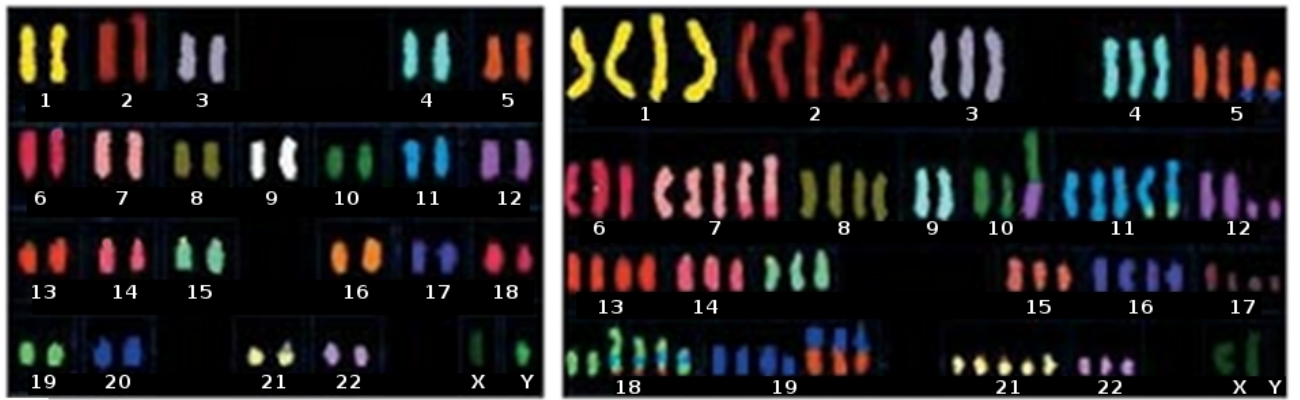
\includegraphics[width=\textwidth]{Karyo-both}
\vskip 0.1in
  \begin{minipage}{0.4\linewidth}
    Normal cell with 2 copies of each autosome.
  \end{minipage}
\hskip 0.1\linewidth
  \begin{minipage}{0.4\linewidth}
Cancer cell with many copy number alterations.
  \end{minipage}

\end{frame}

\begin{frame}
  \frametitle{Unsupervised, non-interactive DNA copy number analysis}
  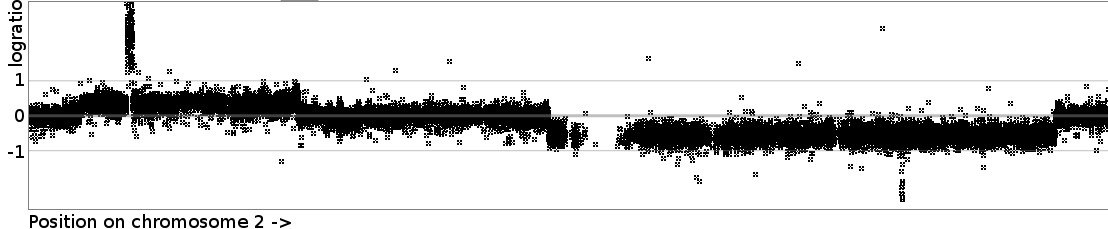
\includegraphics[width=\textwidth]{unlabeled-axes}

  Analyst sees a vector of $d$ noisy data points $\mathbf x\in\RR^d$.

  \vskip 0.1in

  \textbf{Question:}\\
  where are the true changes in copy
  number? (breakpoints)

\end{frame}

\begin{frame}
  \frametitle{Unsupervised, non-interactive DNA copy number analysis}

  \textbf{Usual solution:} fit a statistical model $f(\mathbf x, \theta)$.\\
  ($\theta$ is a model parameter, for example a p-value threshold or
  the number of breakpoints)

  TODO: figure with data, parameters, model.

  \textbf{Problem}: how do we know the model $f$ and parameter
  $\theta$ are reasonable? \textbf{Solution:} plot it!
\end{frame}

\begin{frame}
  \frametitle{Unsupervised, interactive DNA copy number analysis}
  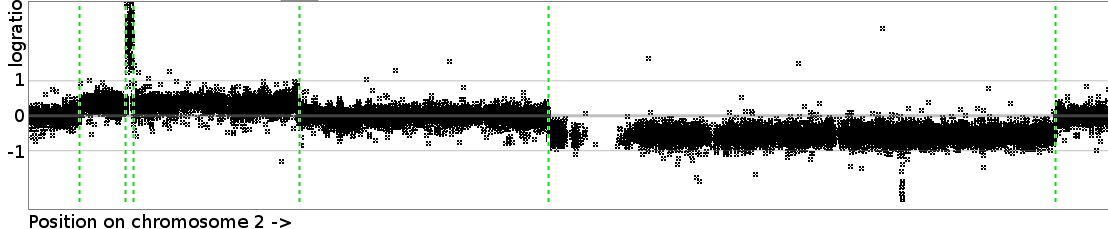
\includegraphics[width=\textwidth]{unlabeled-breakpoints-6}

  Parameter $\theta$ = 6 breakpoints.
\end{frame}

\begin{frame}
  \frametitle{Unsupervised, interactive DNA copy number analysis}
  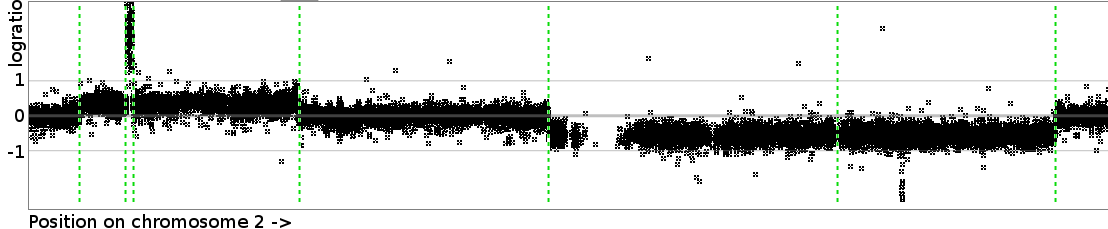
\includegraphics[width=\textwidth]{unlabeled-breakpoints-7}

  Parameter $\theta$ = 7 breakpoints.
\end{frame}

\begin{frame}
  \frametitle{Unsupervised, interactive DNA copy number analysis}
  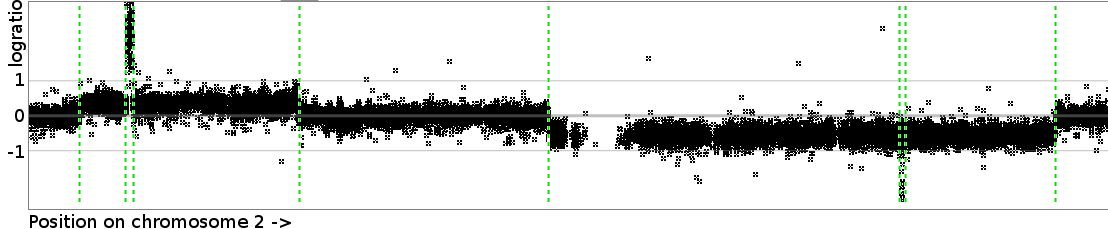
\includegraphics[width=\textwidth]{unlabeled-breakpoints-8}

  Parameter $\theta$ = 8 breakpoints.
\end{frame}

\begin{frame}
  \frametitle{Unsupervised, interactive DNA copy number analysis}
  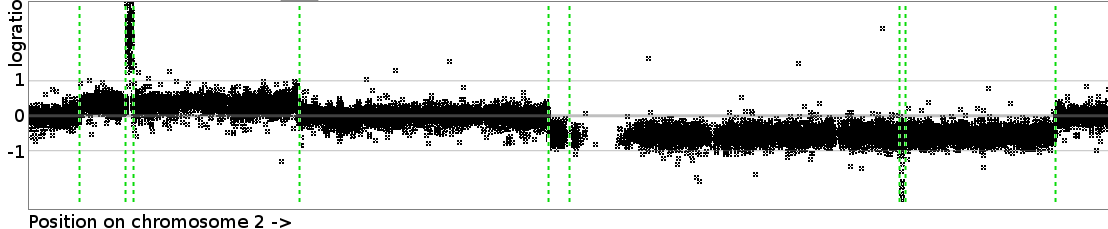
\includegraphics[width=\textwidth]{unlabeled-breakpoints-9}

  Parameter $\theta$ = 9 breakpoints.
\end{frame}

\begin{frame}
  \frametitle{Unsupervised, interactive DNA copy number analysis}
  
  Choose $\theta$ by 

  TODO: figure with data, parameters, model, plot.
\end{frame}

\begin{frame}
  \frametitle{Unsupervised, interactive DNA copy number analysis\\
  with several profiles}
  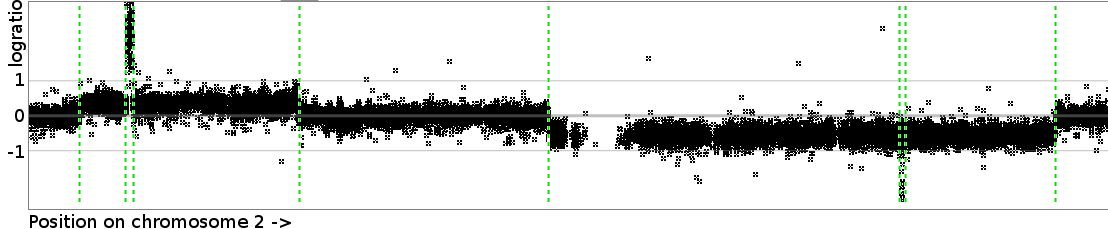
\includegraphics[width=\textwidth]{unlabeled-breakpoints-8}

  Parameter $\theta_1$ = 8 breakpoints.

  \vskip 0.1in

  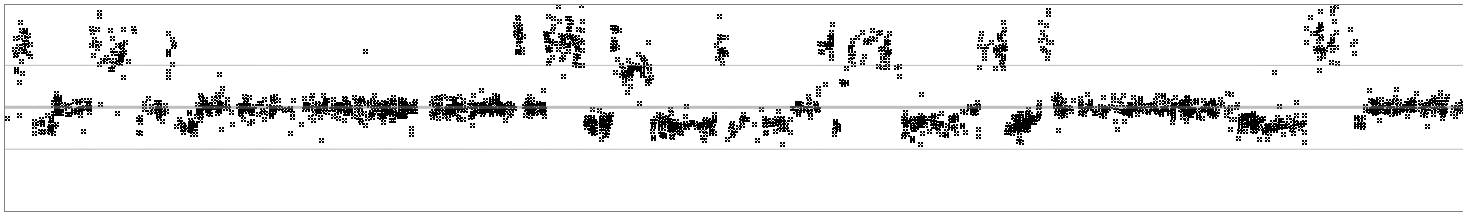
\includegraphics[width=\textwidth]{lots-of-breaks}

  Parameter $\theta_2$ = ??

  \vskip 0.1in

  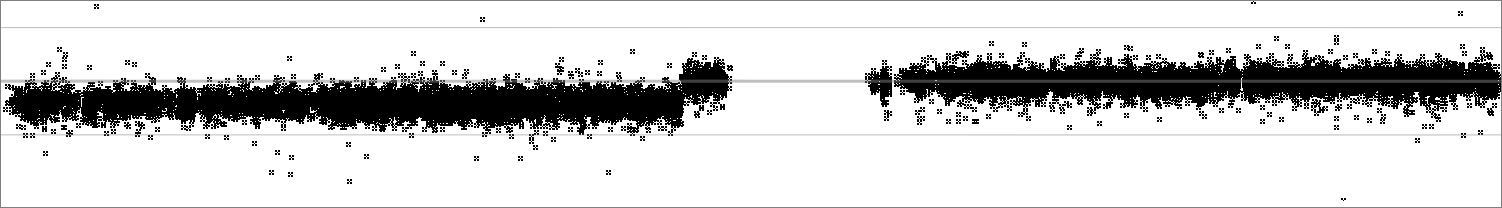
\includegraphics[width=\textwidth]{only-one-break}

  Parameter $\theta_3$ = ??

\end{frame}

\begin{frame}
  \frametitle{Some problems with unsupervised analysis}
  \begin{itemize}
  \item How does the parameter for one profile $\theta_1$ help us
    choose a parameter $\theta_2, \theta_3$ for other profiles?
  \item What if we use a different model $g(\mathbf x, \rho)$ where
    the learned $\theta$ is meaningless?
  \item How to compare two models of the same data? Are the
    breakpoints of $f(\mathbf x, \theta$) or $g(\mathbf x, \rho)$
    better? 
  \end{itemize}

  All of these problems can be solved by supervised learning.
\end{frame}

\section{Supervised DNA copy number analysis}

\begin{frame}
  \frametitle{Computer vision: look and add labels to...}
  \begin{tabular}{ccc}
    Photos & Cell images & Copy number profiles \\
    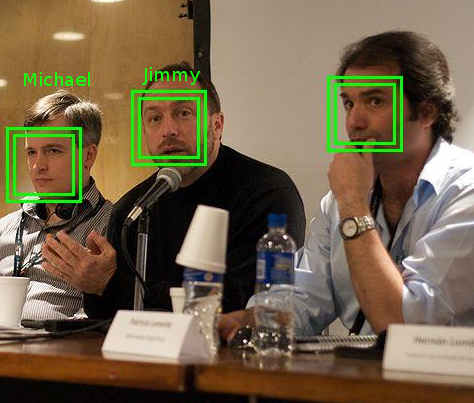
\includegraphics[width=1.3in]{faces} &
    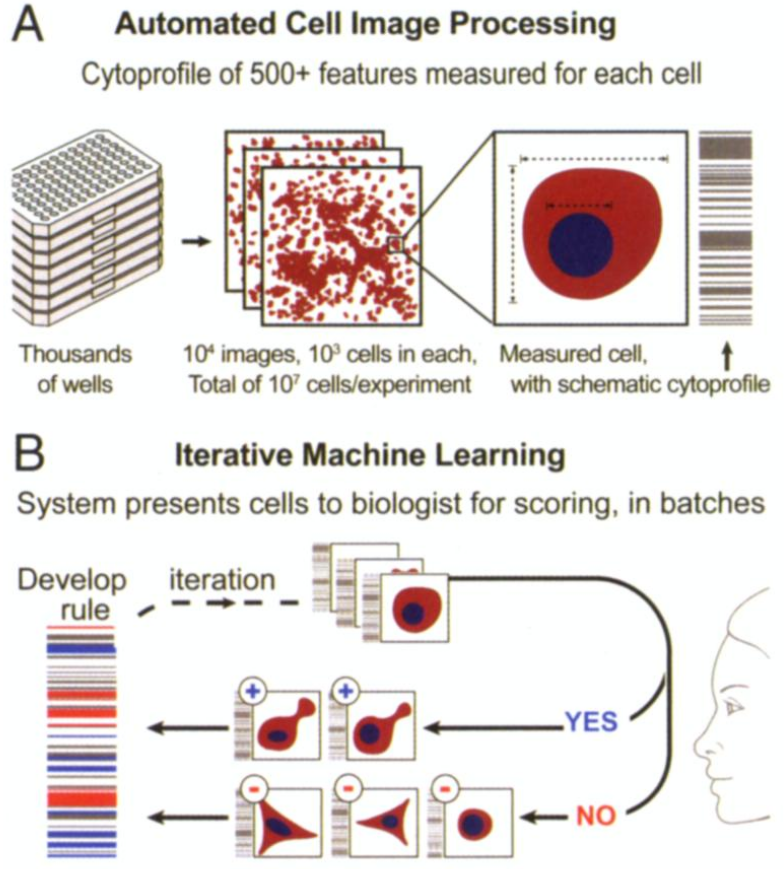
\includegraphics[width=1.3in]{cellprofiler} &
    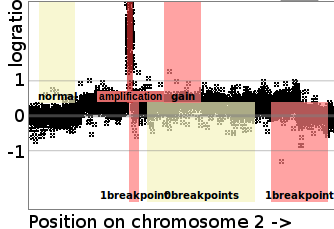
\includegraphics[width=1.5in]{regions-axes}\\
    Labels: names & phenotypes & alterations
  \end{tabular}
  Sources: \url{http://en.wikipedia.org/wiki/Face_detection}\\
  Jones et al PNAS 2009. Scoring diverse cellular morphologies in
  image-based screens with iterative feedback and machine learning.
\end{frame}

\begin{frame}
  \frametitle{Computer vision for genomic segmentation}
  \begin{tabular}{rll}
    \textbf{Breakpoint}\\
 \textbf{detector} & \textbf{strong point} & \textbf{weak point} \\
    \hline
    mathematical  & maximum likelihood & tuning parameters \\
    models & algorithm finds exact  & chosen using\\
& breakpoint locations  & unrealistic assumptions\\
    \hline
    your eyes & outliers, signal/noise & finding the \\
    & over large regions &  exact breakpoint
  \end{tabular}
\vskip 1cm
\textbf{SegAnnDB exploits the strong points of both:}
\begin{itemize}
\item Plot a maximum likelihood model alongside the data.
\item Edit annotated regions.
\item The model parameters are automatically updated to agree.
\item No tuning parameters, but need to annotate a few profiles.
\end{itemize}
Demo on \url{http://bioviz.rocq.inria.fr/}
\end{frame}

\begin{frame}
  \frametitle{Annotated regions allow supervised and interactive models}
  \begin{tabular}{c|c|c|c}
    Evaluation: & qualitative & quantitative \\
    Input: data + & parameters & annotated regions & Plot/update?\\
    \hline
    & \textbf{unsupervised} & \textbf{supervised} & no\\
    & default & params chosen to \\
    & params & agree w/regions\\
    \hline
    & \textbf{tweaked} & \textbf{interactive} & yes\\
    & params & edit regions
  \end{tabular}
  \begin{description}
  \item[2004-now] dozens of \textbf{unsupervised} models that can be
    \textbf{tweaked} e.g. GLAD, DNAcopy, fused lasso, cghseg, PELT.
  \item[2009-2010] Janoueix-Lerosey, Schleiermacher, et al. J Clinical
    Oncology. Breakpoint region labels recorded by typing 0/1 in Excel
    spreadsheets.
  \item[2013] Hocking et al. BMC Bioinformatics protocols for training
    \textbf{supervised} models.
  \item[2014?] paper about SegAnnDB software for \textbf{interactive}
    genomic segmentation under review, Bioinformatics.
  \end{description}
\end{frame}

\begin{frame}
  \frametitle{Supervised, interactive copy number analysis (SegAnnDB)}

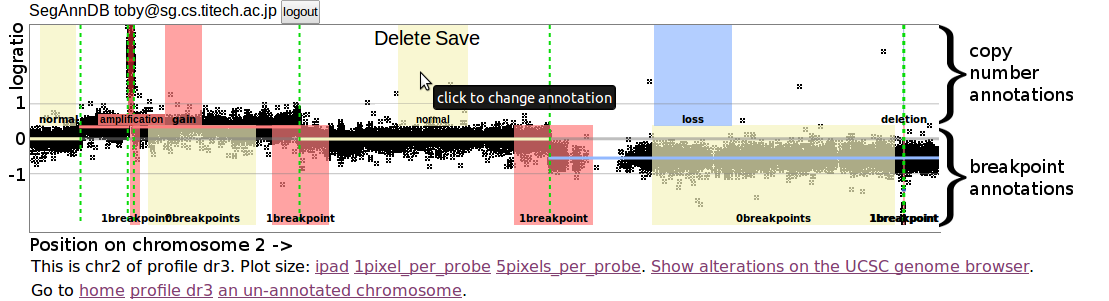
\includegraphics[width=\textwidth]{new-new-annotations}

\vskip 0.2in
Public SegAnnDB server: \url{http://bioviz.rocq.inria.fr/}

\vskip 0.1in
Private server for McGill data sets:
\small
\url{http://ec2-54-201-171-12.us-west-2.compute.amazonaws.com/}

\end{frame}

\begin{frame} 
  \frametitle{Advantages of supervised learning}
  Creating annotation databases is important for
  \begin{description}
  \item[short-term] quantitative evaluation, more convincing papers.
  \item[long-term] cross-discipline collaboration!
    \begin{description}
    \item[statisticians/modelers] get better evaluation
    metrics.
    \item[biologists/annotators] get
    better models.
    \end{description}
  \end{description}
  TODO: all models are false, but some models are useful.

  Can we make labels/supervised approaches for...
  \begin{description}
  \item[segmentation] breakpoint/copy number regions (this work).
  \item[clustering] pairs that should join (or not)?
  \item[regression] variables/genes that are important (or not)?
  \item[diff expression] genes that are up/down (or not)?
  \end{description}
  Write me at \texttt{toby.hocking@mail.mcgill.ca} to collaborate!
\end{frame}

\section{Supervised ChIP-seq peak detection}



\begin{frame}
  \frametitle{Thank you!}
  Supplementary slides appear after this one.
\end{frame}

\end{document}
